\section{AppCoins: Protocol Definition}

As we have seen before, AppCoins protocol addresses the use cases of Advertising, In-App Billing (IAB) and Developer Reputation within App Stores by leveraging the blockchain construction to create value for the different participants.\\

In this section, we present the data structures and algorithms used to solve each of the aforementioned use cases. It will be organised as follows: a section for each core flow and subsections explaining the data structures, algorithms and wallets flows.

\subsection{Advertising}

Advertising campaigns in the context of a blockchain construction must be constructed in a way to overcome the following problems:
\begin{itemize}
\item \textit{Double attribution problem}: For all instances of the same bid (explained in \ref{sssec:ads_ds}) in different App Stores, a user can only be attributed once.
\item \textit{Bid refutation}: A developer must not be able to state that he did not create a bid if it is not true.
\item \textit{Bid validation}: A developer must be able to confirm that the attribution rules match the ones submitted at campaign (explained in \ref{sssec:ads_ds}) creation time.
\end{itemize}

\subsubsection{Data Structures} \label{sssec:ads_ds}

%\noindent \textbf{Campaign}. A \textit{campaign} is a statement of intent to pay for the attention of users. Developers create \textit{campaigns} and submit them to App Stores, which in turn match and propagate them to users. Campaigns are composed by an amount of funds, a duration, the amount of tokens per attribution, and the filters (app name, app version, geolocation,...). Please refer to Table \ref{table: data_structures_ad} for more details. \\
%
%\noindent \textbf{Bid}. A \textit{bid} is a mapping between developers and the users in an App Store that match specific campaigns created by developers. It also contains the funds available for the \textit{bid} and the amount of tokens per attribution, and its duration.\\

\noindent \textbf{Bid}. A \textit{bid} is a statement of intent to pay for the attention of users. Developers create \textit{bids} and submit them to App Stores, which in turn match and propagate them to users. Bids are composed by an amount of funds, a duration, the amount of tokens per attribution, the filters (app name, app version, geolocation,...). and a mapping between developers and the users in an App Store that match specific filters set by the developers. Please refer to Table \ref{table: data_structures_ad} for more details. \\

\noindent \textbf{Inverted bid}. An \textit{inverted bid} is a mapping between users and the bids they are participating in for a specific app store. See Table \ref{table: data_structures_ad} for more details.\\

\noindent \textbf{Advertising Ledger}. The \textit{advertising ledger} is the record of attributions, i.e. users that did the required action (e.g. having an app open for at least 2 minutes) for a bid. The ledger is populated in a way that avoids the \textit{double attribution problem}, i.e. bids in different App Stores for the same apps in similar time intervals need to be identifiable across all the stores, as well as the users.

%\begin{table}[H]
%\footnotesize
%\centering
%\begin{tabular}{|p{.5\textwidth}p{.5\textwidth}|}
%\hline
%\multicolumn{2}{|c|}{Data Structures} \\
%\hline \vspace{0.05cm}
%\textbf{Campaign} & \vspace{0.05cm} \textbf{Bid} \\
%campaign $C_{ij} := \langle F_{ij}, \Delta t_{ij}, T_{ij}, filters \rangle_{D_{i}, AP_{j}}$
%\begin{itemize}
%	\item Funds $F_{ij}$, the amount of tokens the developer $D_{i}$ is willing to spend for $C_{ij}$ in an app store $AP_{j}$
%	\item Duration $\Delta t_{ij}$, the duration of $C_{ij}$ in $AP_{j}$
%	\item Tokens per attribution $T_{ij}$, the amount of tokens to be sent from $D_{i}$ and distributed to the other parties per attribution
%	\item Filters, the specifics of $C_{ij}$, as the app name, app version, geolocation of $C_{ij}$, and others available to $D_{i}$
%\end{itemize}
%& bid $B_i : \{D_1 \to (U_1..U_n)\}_{AP_j}$
%why D_1 instead of D_i?
%add relationship between B and C? 
%\begin{itemize}
%	\item Developer $D_i$, developer that submitted a bid $B_i$ to the app store $AP_j$ 
%	\item User $U_i$, user matching the filters of campaign $C_{ij}$ associated with bid $B_i$ in app store $AP_j$
%\end{itemize} \\
%\textbf{Inverted Bid} & \textbf{Advertising Ledger} \\
%inverted bid $IB_i : \{U_1 \to (B_1..B_n), U_2..\}_{AP_j}$
%\begin{itemize}
%	\item User $U_i$, user matching one or more bids $B_{i..n}$ in app store $AP_j$
%	\item Bid $B_i$, bids submitted to app store $AP_j$
%\end{itemize}
%& advertising ledger $L_{Ad} : (A^{1}_{t}..A^{n}_{t})$
%\begin{itemize}
%	\item Attribution $A^{i}_{t}$, $i$-th attribution in the advertising ledger $L$, which is composed as a mapping $A^{i}_{t} : \{B_{N}^{j} \to (U_{N}^{1}..U{N}^{n})\}$, where $B_{N}^{j}$ is the standardised bid $B_j$ across all the app stores where it is defined and $U_{N}^{i}$ is the normalised user $U_i$ across all the app stores
%\end{itemize} \\
%\hline
%\end{tabular}
%\caption{Data Structures for Advertising Use Case}
%\label{table: data_structures_ad}
%\end{table}
\begin{table}[H]
\footnotesize
\centering
\begin{tabular}{|p{.5\textwidth}p{.5\textwidth}|}
\hline
\multicolumn{2}{|c|}{Data Structures} \\
\hline \vspace{0.05cm}
\textbf{Bid} & \vspace{0.05cm} \textbf{Inverted Bid} \\
bid $B_i : \langle F_{ij}, \Delta t_{ij}, T_{ij}, filters, D_1 \to (U_1..U_n) \rangle_{D_{i}, AP_{j}}$
%add introduction to i.j indexes?
%why \Delta t_{ij} has ij? does it time relate appstore and user or is it related to the bid (e.g. store with multiple bids what does it mean)?
\begin{itemize}
	\item Funds $F_{ij}$, the amount of tokens the developer $D_{i}$ is willing to spend for $C_{ij}$ in an app store $AP_{j}$
	\item Duration $\Delta t_{ij}$, the duration of $C_{ij}$ in $AP_{j}$
	\item Tokens per attribution $T_{ij}$, the amount of tokens to be sent from $D_{i}$ and distributed to the other parties per attribution
	\item Filters, the specifics of $C_{ij}$, as the app name, app version, geolocation of $C_{ij}$, and others available to $D_{i}$
	\item Developer $D_i$, developer that submitted a bid $B_i$ to the app store $AP_j$ 
	\item User $U_i$, user matching the filters of campaign $C_{ij}$ associated with bid $B_i$ in app store $AP_j$
\end{itemize} &
inverted bid $IB_i : \{U_1 \to (B_1..B_n), U_2..\}_{AP_j}$
\begin{itemize}
	\item User $U_i$, user matching one or more bids $B_{i..n}$ in app store $AP_j$
	\item Bid $B_i$, bids submitted to app store $AP_j$
\end{itemize} \\
\textbf{Advertising Ledger} & \\
advertising ledger $L_{Ad} : (A^{1}_{t}..A^{n}_{t})$
%what is the index t?
\begin{itemize}
	\item Attribution $A^{i}_{t}$, $i$-th attribution in the advertising ledger $L$, which is composed as a mapping $A^{i}_{t} : \{B_{N}^{j} \to (U_{N}^{1}..U{N}^{n})\}$, where $B_{N}^{j}$ is the standardised bid $B_j$ across all the app stores where it is defined and $U_{N}^{i}$ is the normalised user $U_i$ across all the app stores
\end{itemize} & \\
\hline
\end{tabular}
\caption{Data Structures for Advertising Use Case}
\label{table: data_structures_ad}
\end{table}


\subsubsection{Algorithms' Pseudo-code}

Table \ref{table: ads_use_case} presents in pseudo-code a more in-depth definition of the following methods. \\

\noindent \textbf{Create bid}. When a bid is submitted to the App Store, the \textsf{CreateBid} method creates the bid $B$ containing the mapping $M$ between the developer $D$ and the set of users $U$ of the app store that match the filters, as well as all the parameters describing the bid as the funds $F$, duration $\Delta t$, etc. The inverted bids $IB_{i...n}$ of the app store containing the mapping between users and the bids they are in are created or updated, if they already exist. In addition, the funds $F$ the developer wishes to allocate to the campaign are sent from the developer's wallet $W_D$ to the bid's contract wallet $W_B$. Since the created bid is in the blockchain accessible to every user, it is used to overcome the \textit{bid refutation} problem.\\

\textsf{AD.CreateBid}
\begin{itemize}
	\item INPUTS:
	\begin{itemize}
		\item Campaign parameters:
		\begin{itemize}
			\item Funds $F$
			\item Duration $\Delta t$
			\item Tokens paid per attribution $T$
			\item Filters (geolocation, app name, app version,...)
		\end{itemize}
		\item Developer $D$
		\item App Store $AS$ %App Store was AP in previous definitions
	\end{itemize}
	\item OUTPUTS: Bid $B$ and inverted bid $IB$
\end{itemize}

\noindent \textbf{Validate bid}. When a bid is to be shown to the user $u$, \textsf{ValidateBid} validates that bid in the blockchain to confirm if it is a valid bid and if the user $u$ matches its filters. In order to avoid the scenario where there are not enough funds available in the bid for the user, the tokens per attribution $T$ defined in the bid are sent to the bid's captivation wallet $W_C$ for a period of time. The method is used to overcome the problem of \textit{bid validation}. \\

\textsf{AD.ValidateBid}
\begin{itemize}
	\item INPUTS:
	\begin{itemize}
		\item User $u$
		\item App Store $AS$
	\end{itemize}
	\item OUTPUTS: Result $R$ (0 or 1)
\end{itemize}

\noindent \textsf{Set attribution}. When a user has been attributed to a bid $B$, i.e. the user performed the required action (e.g. had the app open for at least 2 minutes), \textsf{SetAttribution} checks the advertising ledger $L_{Ad}$ to make sure the user $u$ has not yet been attributed to the bid $B$ and if so, the attribution is written in the ledger and each participant receives the correspondent tokens, i.e. the user, OEM and app store receive $T_u$, $T_{OEM}$ and $T_{AS}$, respectively. Since the method is constructed in a way such that the same user is unable to be attributed the same bid in different app stores, it avoids the \textit{double attribution problem}. \\

\textbf{AD.SetAttribution}
\begin{itemize}
	\item INPUTS:
	\begin{itemize}
		\item User $u$
		\item Bid $B$
	\end{itemize}
	\item OUTPUTS: Result $R$ (0 or 1)
\end{itemize}

\begin{table}[H]
\scriptsize
\centering
\begin{tabular}{|p{.5\textwidth}p{.5\textwidth}|}
\hline
\multicolumn{2}{|c|}{Advertising Use Case} \\
\hline \vspace{0.1cm}
\textsf{AD.CreateBid}
\begin{itemize}
	\vspace{-0.3cm}
	\item INPUTS:
	\vspace{-0.4cm}
	\begin{itemize}
		\item Campaign parameters:
		\begin{itemize}
			\item Funds $F$
			\item Duration $\Delta t$
			\item Tokens paid per attribution $T$
			\item Filters (geolocation, app name,...)
		\end{itemize}
		\item Developer $D$
		\item App Store $AS$
	\end{itemize}
	\item OUTPUTS: Bid $B$ and inverted bid $IB$
\end{itemize}
\begin{enumerate}
	\item Compute $U$ := \textsf{GetUsers}($AS$, $filters$)
	\item Compute $M$ := \textsf{Mapping}($D$, $U$)
	\item Compute $B$ := \textsf{CreateBid}($F$, $D$, $\Delta t$, $T$, $filters$, $M$)
	\item Send $F$ from developer's wallet $W_D$ to bid's wallet $W_B$
	\item For each $u$ in $U$:
	\vspace{-0.3cm}
	\begin{enumerate}
		\item Compute $IB_u$ := \textsf{GetIB}($u$)
		\item If $IB_u = -1$: 
		\begin{enumerate}
			\item Compute $IB_u$ := \textsf{CreateIB}($u$)
		\end{enumerate}
		\item Else:
		\begin{enumerate}
		 \item Compute $IB_u$.\textsf{append}($B$)
		\end{enumerate}
	\end{enumerate}
\end{enumerate} & \vspace{0.1cm} \textsf{AD.SetAttribution}
\begin{itemize}
	\vspace{-0.3cm}
	\item INPUTS:
	\vspace{-0.4cm}
	\begin{itemize}
		\item User $u$
		\item Bid $B$
	\end{itemize}
	\item OUTPUTS: Result $R$
\end{itemize}
\begin{enumerate}
	\item Compute $InLedger$ := \textsf{CheckAdvertisingLedger}($u$, $B$)
	\item If $InLedger$ = 1:
	\begin{itemize}
		\item Set $R$ := 0
	\end{itemize}
	\item If $InLedger$ = 0:
	\begin{enumerate}
		\item Compute $TX$ := \textsf{Transaction}($u$, $B$)
		\item Compute $R$ := \textsf{WriteAdvertisingLedger}($TX$)
		\item Compute $(T_u, T_{OEM}, T_{AS})$ := \textsf{DivideTokens}($T$)
		\item Send $T_u$ to user's wallet $W_U$
		\item Send $T_{OEM}$ to OEM's wallet $W_{OEM}$
		\item Send $T_{AS}$ to user's wallet $W_{AS}$
	\end{enumerate}
\end{enumerate} \\
\textsf{AD.ValidateBid}
\begin{itemize}
	\vspace{-0.3cm}
	\item INPUTS:
	\vspace{-0.4cm}
	\begin{itemize}
		\item User $u$
		\item App Store $AS$
	\end{itemize}
	\item OUTPUTS: Result $R$
\end{itemize}
\begin{enumerate}
	\item Compute $B^{'}_{u}$ := \textsf{GetBids}($u$, $AS$)
	\item Compute $IB_u$ = \textsf{GetIB}($u$)
	\item Set $IB^{'}_{u}$ := $\{u \to (B^{'1}_{u}..B^{'n}_{u}) = B^{'}_{u}\}$
	\item Compute $R$ := \textsf{CheckMatch}($IB_u$, $IB^{'}_{u}$)
	\item If $R = 1$:
	\begin{enumerate}
		\item Send $T$ from bid's wallet $W_B$ to bid captivation wallet $W_C$
	\end{enumerate}
\end{enumerate} & \\
\hline
\end{tabular}
\caption{Advertising Use Case}
\label{table: ads_use_case}
\end{table}


\subsubsection{Wallets' Transactions}

The transfers between wallets in the Advertising flow have to address some risks that were previsously decribed in chapter ...%missing reference

There is a wallet that contains the value of the created campagin, addressing the risk of ...%missing text

There is a wallet temporarilly storing the value of the impression, to be sure that if the conversion occurs, the conversion is payed.

\begin{figure}[!ht]
\centering
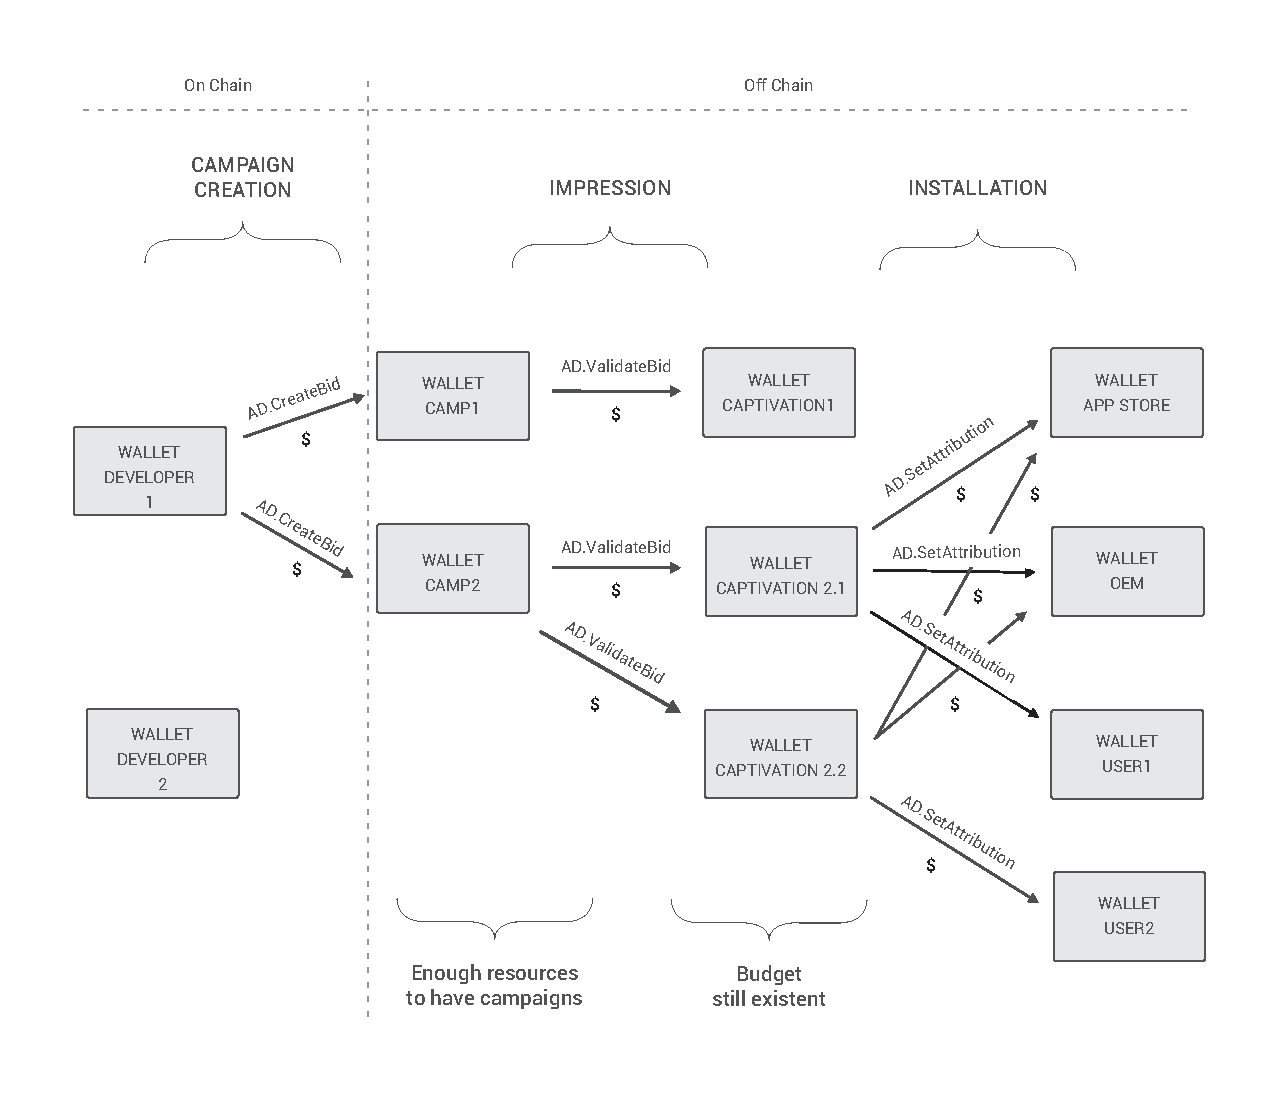
\includegraphics[width=\textwidth]{diagrams/wallet_transfers.eps}
\caption{Wallet transfers in the CPI advertising flow.}
\label{fig:wallet_cpi_flow}
\end{figure}


% todo complete the text after the diagram is ready


\subsection{In-App Billing}
%missing intro?

\subsubsection{Data Structures}

\noindent \textbf{Catalog}. A \textit{catalog} is a mapping between items available in an app and their prices. Each item has only one price and the mapping is bonded to an App Store, i.e. the price can be set differently for different App Stores. \\

\noindent \textbf{IAB Ledger}. The \textit{IAB ledger} is the record of items bought by users. It records transactions in a way that anyone can verify an anonymous user bought a quantity $Q$ of an item $I$ for a price $P$ from an app that integrated the IAB solution from App Store $AS$. %App Store was previously defined AP

\begin{table}[H]
\footnotesize
\centering
\begin{tabular}{|p{1.0\textwidth}|}
\hline
\multicolumn{1}{|c|}{Data Structures} \\
\hline \vspace{0.05cm}
\textbf{Catalog} \\
catalog $C_{ij} : \{I_1 \to P_1..I_n \to P_n\}_{A_i, AS_j}$
%C was campaign, would be better to chose different symbol
\begin{itemize}
	\item Item $I_i$, an item available in app $A_i$ which integrated IAB solution from app store $AS_j$
	\item Price $P_i$, the price of item $I_i$
\end{itemize} \\
\textbf{IAB Ledger} \\
IAB ledger $L_{IAB} : (TX_1..TX_n)$
\begin{itemize}
	\item Transaction $TX_i$, a transaction stating that an anonymous user $u$ bought a quantity $Q$ an item $I$ with price $P$ from an app $A$ that integrated the IAB solution from app store $AS$
\end{itemize} \\
\hline
\end{tabular}
\caption{Data Structures for IAB Use Case}
\label{table: data_structures_iab}
\end{table}


\subsubsection{Algorithms' Pseudo-code}


\noindent \textbf{Create catalog}. When a developer $D$ wants to integrate in-app purchases, a catalog $C$ is created containing the mapping between the items $I_N$ that are to be available in the app $A$ and their respective prices $P_N$. \\

\textsf{IAB.CreateCatalog}
\begin{itemize}
	\item INPUTS:
	\begin{itemize}
		%N previously used as normalized?
		\item Set of items $I_N = (I_1..I_n)$
		\item Set of prices $P_N = (P_1..P_n)$
		\item App $A$
		\item App store $AS$
	\end{itemize}
	\item OUTPUTS: Catalog $C$
\end{itemize}

\noindent \textsf{Create transaction}. When a user $u$ wants to buy a certain amount $Q$ of items $I$, a transaction is created stating that the user $u$ bought a quantity $Q$ of an item $I$ for a price $P$ in a app $A$ that integrated the IAB solution from app store $AS$. \\

\textsf{IAB.CreateTransaction}
\begin{itemize}
	\item INPUTS:
	\begin{itemize}
		\item User $u$
		\item Item $I$
		\item Quantity $Q$
		\item App $A$
		\item App store $AS$
	\end{itemize}
	\item OUTPUTS: Result $R$ (0 or 1)
\end{itemize}

\begin{table}[H]
\scriptsize
\centering
\begin{tabular}{|p{0.45\textwidth}p{0.55\textwidth}|}
\hline
\multicolumn{2}{|c|}{IAB Use Case} \\
\hline \vspace{0.1cm}
\textsf{IAB.CreateCatalog}
\vspace{-0.3cm}
\begin{itemize}
	\item INPUTS:
	\vspace{-0.4cm}
		\begin{itemize}
		\item Set of items $I_N = (I_1..I_n)$
		\item Set of prices $P_N = (P_1..P_n)$
		\item App $A$
		\item App store $AS$
	\end{itemize}
	\item OUTPUTS: Catalog $C$
\end{itemize}
\begin{enumerate}
	\item Compute $M$ := \textsf{Mapping}($I_N$, $P_N$)
	\item Compute $C$ := \textsf{Catalog}($M$, $A$, $AS$)
\end{enumerate} & 
\vspace{0.1cm} \textsf{IAB.CreateTransaction}
\vspace{-0.3cm}
\begin{itemize}
	\item INPUTS:
	\vspace{-0.4cm}
	\begin{itemize}
		\item User $u$
		\item Item $I$
		\item Quantity $Q$
		\item App $A$
		\item App store $AS$
	\end{itemize}
	\item OUTPUTS: Result $R$ (0 or 1)
\end{itemize}
\begin{enumerate}
	\item Compute $TX$ := \textsf{Transaction}($u$,$I$,$P$,$Q$,$A$, $AS$)
	\item Compute $R$ := \textsf{WriteIABLedger}($TX$)
	\item if $R = 1$:
	\begin{enumerate}
		\item App $A$ issues items to user
		\item Compute $(T_D, T_{OEM}, T_{AS})$ := \textsf{DivideTokens}($F$)
		\item Send $T_D$ to developer's wallet $W_D$
		\item Send $T_{OEM}$ to OEM's wallet $W_{OEM}$
		\item Send $T_{AS}$ to user's wallet $W_{AS}$
	\end{enumerate}
\end{enumerate} \\
\hline
\end{tabular}
\caption{IAB Use Case. In \textsf{CreateTransaction}, the issuing of items in certain app $A$ is purely done in the app based on the result of the method, since the items are not in the blockchain and there is no real blockchain transaction happening.}
\label{table: iab_protocol}
\end{table}

\subsection{Developers' Rank}

There is the need to create trust between the different players in the app economy, namely between users, the developers and their apps. \\

In the AppCoins protocol, trust is characterised by a developer's rank, which is then propagated to all his apps. This rank can have the values of $\{"Unknown", "Trusted", "Critical"\}$. A user has the rank \textit{"Unknown"} only when joining the network for the first time, i.e. once the rank is changed from \textit{"Unknown"}, it can never have this value again. Changes in rank happen by either disputes, where the rank of the developer can change to \textit{"Critical"} in case of loss or remain the same in case of win, or by promotions, where the rank of the developer can change to \textit{"Trusted"}.

Promotions depend on the number of transactions in each of the developer's apps compared to the number of transactions in other popular apps. Promotions are automatic and depend on the following condition:

\begin{equation}
\sum\limits_{t=0}^{T} \sum\limits_{i=1}^{N} TX_{A_{ij},t} \geq TX_{A^{T}_{M}}
%T variable in the date and part of TX is confusing looks like T multiplied by X
\label{eq: promo_cond}
\end{equation}

where $A_i = \{A_{i1}..A_{iN}\}$ is the set of N apps of developer $D_i$, meaning that $A_{ij}$ is the app $j$ in the set $A_i$, $t$ is the day with $t=0$ being the moment the developer joined the network, $T$ is the current day, $A^{T}_{M}$ is the app with the highest number of transactions on day $T$. Given these variables definitions, one can see that the left side in Equation \ref{eq: promo_cond} represents the amount of transactions in all the apps of developer $D_i$ since he joined the network, and the right side represents the number of transactions of the app with the highest number of transactions on day $T$.

Contrary to the promotions, disputes are not done automatically and require explicit actions from users. Any user can open a dispute with a developer stating that the developer is dishonest. After the dispute is opened, any other user can join either side, depending on if they want to support the accusation of dishonesty or if they want to defend the developer.

Additionally, each rank value has a level associated with it. For \textit{"Unknown"} and \textit{"Critical"} rank values, the level is always set to 1. When the rank is \textit{"Trusted"}, we do not set a maximum level and it is expressed by:
\begin{equation}
S_l = \log_2 \frac{\sum\limits_{t=0}^{T} \sum\limits_{i=1}^{N} TX_{A_{ij},t}}{TX_{A^{T}_{M}}}
\label{eq: rank_level}
\end{equation}

Because of the use of the logarithm function in Equation \ref{eq: rank_level}, it becomes harder to gain higher rank levels as the rank level increases.


\subsubsection{Wallets' Transactions}

In In-App Billing the transactions between wallets occur off-chain. The main transactions are between the user that is buying the digital item and 3 recipients: the developer, the OEM and the app store.


\subsection{Developers' Reputation}

A known developer is more trustable than a developer recently arrived to the apps' distribution business.

In figure \ref{fig:approval_state_diagram}, the different states that the developer can have are presented.

\begin{figure}[!ht]
\centering
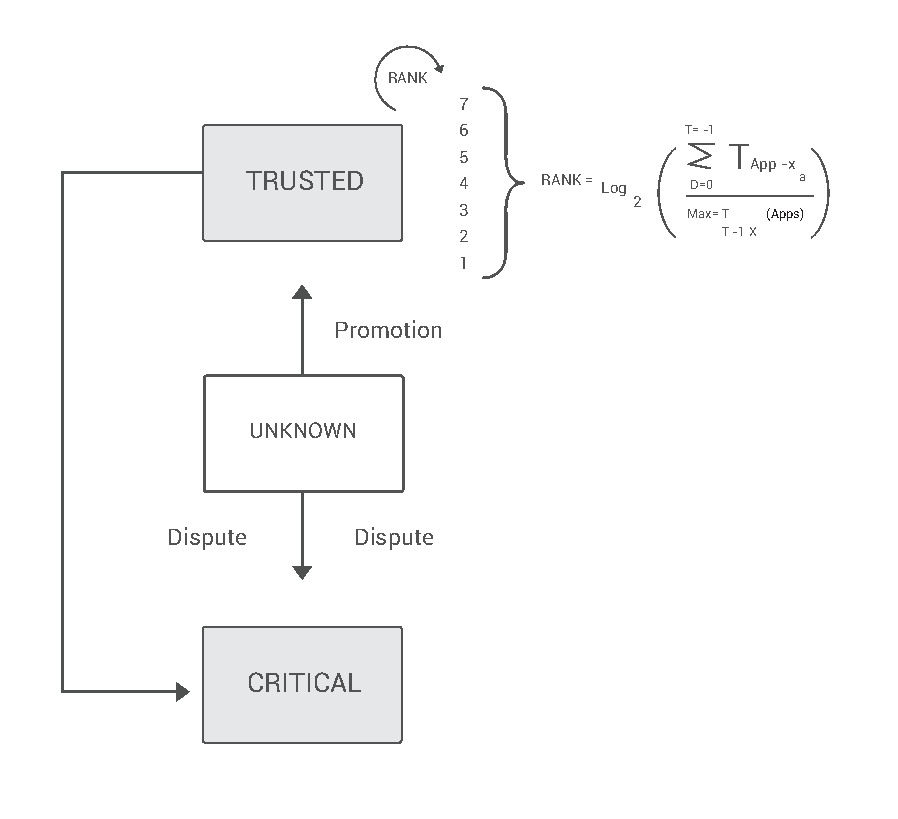
\includegraphics[width=0.5\textwidth]{diagrams/approval_state_diagram.eps}
\caption{Approval state changes.}
\label{fig:approval_state_diagram}
\end{figure}


\subsubsection{Data Structures}

\noindent \textsf{Dispute Intent}. A \textit{dispute intent} happens when a user claims that a developer is dishonest and no dispute against that developer is open. The developer or any other user then has 7 days to answer the dispute. If someone answers the dispute, be it the developer or any other user, the dispute is opened and the minimum fees needed to open it are captivated. If no user answers the dispute, the \textit{dispute intent} closes and the developer status changes to \textit{critical}. \\
%in the last sentence "If no user answers the dispute". Shouldn't it be "If no user or developer answers the dispute" else a user can allways blacklist any developer provided that other users don't reply

\noindent \textsf{Dispute}. A \textit{dispute} is a conflict between two parties, where one party - the \textit{contestants} - claim that a developer is dishonest, i.e. the developer uploads apps with malware, too many ads, or non-working apps, and the other party - the \textit{pleaders} - claim the developer is honest. The pleaders include the developer being accused of dishonesty by the contestants. Both parties place tokens in the dispute and the party holding the most amount of tokens by the end of the dispute wins. Therefore, the \textit{dispute} includes the developer it regards to, the participants in both parties and their respective stake in the dispute. \\
%how many tokens each user, developer puts?

\noindent \textsf{DisputeLedger}. The \textit{dispute ledger} is the record of users joining disputes. It stores that a user joined a dispute on behalf of one of the sides with a certain stake (amount of tokens). The entries in the \textit{dispute ledger} are used to settle disputes when they end. \\

\noindent \textsf{RankLedger}. The \textit{rank ledger} is the record of rank changes of developers. Whenever there is a change in a developer's rank, be it an increase in the \textit{"Trusted"} rank levels or a change to \textit{"Critical"}, it is recorded in the \textit{rank ledger}.

\begin{table}[H]
\footnotesize
\centering
\begin{tabular}{|p{1.0\textwidth}|}
\hline
\multicolumn{1}{|c|}{Data Structures} \\
\hline \vspace{0.05cm}
\textbf{DisputeIntent} \\
dispute intent $K^{0}_{x} := \langle D_i, C_j, T_{min}, S\rangle$
\begin{itemize}
	\item Developer $D_i$, the developer being accused of being dishonest
	\item Contestant $C_j$, user claiming developer $D_i$ is dishonest
	%C has been defined as campaign
	\item Minimum fee $T_{min}$, the minimum fee needed to open the dispute that may result from this dispute intent
	\item status $S$, the current status of the dispute intent, which can take the values of \textit{"Open"} or \textit{"Closed"}
\end{itemize} \\
\textbf{Dispute} \\
dispute $K_x := \langle D_i, S, T_{min}\rangle$
\begin{itemize}
	\item Developer $D_i$, the developer being accused of being dishonest
	\item status $S$, the current status of the dispute, which can take the values of \textit{"Open"} or \textit{"Closed"}
	\item Minimum fee $T_{min}$, the minimum fee needed to open the dispute
	%who defines the value of $T_{min}$, dows it change between disputes?
\end{itemize} \\
\textbf{Dispute Ledger} \\
dispute ledger $L_{K} : (E_1..E_n)$
\begin{itemize}
	\item entry $E_i$, an entry containing information about a user joining a dispute in the form $E_i := \langle U_i, P, T, K_x\rangle$, where $U_i$ is the user, $P$ is the position the user is taking (can be either \textit{"Contestants"} or \textit{"Pleaders"}), $T$ is the stake (amount of tokens) the user $U_i$ is willing to use to defend position $P$, and $K_x$ is the dispute user $U_i$ is joining
\end{itemize} \\
\textbf{Rank Ledger} \\
rank ledger $L_{R} : (E_1..E_n)$
\begin{itemize}
	\item entry $E_i$, an entry containing information about a change in a developer's rank in the form $E_i := \langle D_i, S_b, S_a, S_l\rangle$, where $D_i$ is the developer, $S_b$ is the developer's rank before the change, $S_a$ is the rank after the change, and $S_l$ is the level of the rank. $S_b$ can take the values of $\{"Unknown", "Trusted"\}$ and $S_a$ can take the values of $\{"Trusted", "Critical"\}$. For further details regarding the possible states of $S_b$ and $S_a$, and the possible values of $S_l$, please refer to Figure \textbf{[INCLUDE REF TO FIG]}.
\end{itemize} \\
\hline
\end{tabular}
\caption{Data Structures for Developers Rank Use Case}
\label{table: data_structures_da}
\end{table}


\subsubsection{Algorithms' Pseudo-code}

%user was previously $U$
%what are i,j,z,x ans 0
\noindent \textbf{Create dispute intent}. When a user $C_i$ claims a developer $D_j$ is dishonest, an intent of dispute is created, which may result in a dispute being opened, depending on whether someone answers the \textit{dispute intent} within 7 days or not. The user answering the dispute may not be the developer. \\

\textsf{DR.CreateDisputeIntent}
\begin{itemize}
	\item INPUTS:
	\begin{itemize}
		\item User $C_z$
		\item Developer $D_j$
	\end{itemize}
	\item OUTPUTS: Dispute intent $K^{0}_{x}$
\end{itemize}

\noindent \textbf{Create dispute}. When a dispute intent is answered, a disputed is created. Within the following 30 days, any user may join the contestants side, which is composed by users claiming the developer $D_j$ is dishonest, or the pleaders side, which contains users stating that the developer $D_j$ is honest. The dispute intent that originated the new dispute is closed.\\

\textsf{DR.CreateDispute}
\begin{itemize}
	\item INPUTS:
	\begin{itemize}
		\item Developer $D_j$
		\item Minimum fee $T_{min}$
		\item Dispute intent $K^{0}_{x}$
	\end{itemize}
	\item OUTPUTS: Dispute $K_x$
\end{itemize}

\noindent \textbf{Close dispute}. When the dispute is over (after 30 days), the winning side has its stakes refunded, while also receiving 10\% of each pledge from the losing side, with each winning member getting a winning stake proportional to their stake in the overall winning side pledge. Each member from the losing side gets a refund from the respective pledge subtracted by 10\%. Please refer to Table \ref{table: dr_protocol} for more details. \\

\textsf{DR.CloseDispute}
\begin{itemize}
	\item INPUTS:
	\begin{itemize}
		\item Dispute $K_x$
	\end{itemize}
	\item OUTPUTS: None
\end{itemize}

\noindent \textbf{Compute rank}. The rank of the developer is periodically checked to assess changes in its value. For example, the rank can change from \textit{"Unknown"} to \textit{"Trusted"} or the \textit{"Trusted"} level can increase. \\

\textsf{DR.ComputeRank}
\begin{itemize}
	\item INPUTS:
	\begin{itemize}
		\item Developer $D_i$
		\item Set of transactions in developer's apps $TX_i$
		\item Set of developer's apps $A_i$
		\item App with the highest amount of transactions $A_M$
	\end{itemize}
	\item OUTPUTS: None
\end{itemize}

\noindent \textbf{Record dispute}. When a user joins a side on a dispute, the event is recorded in the dispute ledger and can later be used to settle the dispute. \\

\textsf{DR.RecordDispute}
\begin{itemize}
	\item INPUTS:
	\begin{itemize}
		\item User $U_i$
		\item Position $P$
		\item Stake $T$
		\item Dispute $K_x$
	\end{itemize}
	\item OUTPUTS: None
\end{itemize}

\noindent \textbf{Record rank change}. When there is a developer's rank change, it is recorded in the rank ledger. \\

\textsf{DR.RecordRank}
\begin{itemize}
	\item INPUTS:
	\begin{itemize}
		\item Developer $D_i$
		\item New rank $S_a$
		\item New rank level $S_l$
	\end{itemize}
	\item OUTPUTS: None
\end{itemize}

\begin{table}[H]
\scriptsize
\centering
\begin{tabular}{|p{.5\textwidth}p{.5\textwidth}|}
\hline
\multicolumn{2}{|c|}{Developers' Rank Use Case} \\
\hline \vspace{0.1cm}
\textsf{DR.CreateDisputeIntent}
\vspace{-0.3cm}
\begin{itemize}
	\item INPUTS:
	\vspace{-0.3cm}
	\begin{itemize}
		\item User $C_z$
		\item Developer $D_j$
	\end{itemize}
	\item OUTPUTS: Dispute intent $K^{0}_{x}$
\end{itemize}
\begin{enumerate}
	\item Compute $K^{0}_{x}$ := \textsf{DisputeIntent}($D_j$, $C_z$)
	\item Set $K^{0}_{x}$.Status := \textit{"Open"}
\end{enumerate} & \vspace{0.1cm}
\textsf{DR.CreateDispute}
\vspace{-0.3cm}
\begin{itemize}
	\item INPUTS:
	\vspace{-0.3cm}
	\begin{itemize}
		\item Developer $D_j$
		\item Minimum fee $T_{min}$
		\item Dispute intent $K^{0}_{x}$
	\end{itemize}
	\item OUTPUTS: Dispute $K_x$
\end{itemize}
\begin{enumerate}
	\item Set $K^{0}_{x}$.Status := \textit{"Closed"}
	\item Compute $K_x$ := \textsf{Dispute}($D_j$, $T_{min}$)
	\item Set $K_x$.Status := \textit{"Open"}
\end{enumerate} \\ \vspace{0.1cm}
\textsf{DR.CloseDispute} 
\vspace{-0.3cm}
\begin{itemize}
	\item INPUTS:
	\vspace{-0.3cm}
	\begin{itemize}
		\item Dispute $K_x$
	\end{itemize}
	\item OUTPUTS: None
\end{itemize}
\begin{enumerate}
	\item Compute $WinSide$ := \textsf{WinningSide}($K_x$)
	\item Compute \textsf{DistributePledges}($K_x$)
	\item Set $K_x$.Status := \textit{"Closed"}
	\item If $WinSide$ = \textit{"Contestants"}:
	\begin{enumerate}
		\item Compute \textsf{DR.RecordRank}($K_x$.D, \textit{"Critical"}, 1)
	\end{enumerate}
\end{enumerate} & \vspace{0.1cm}
\textsf{DR.ComputeRank} 
\vspace{-0.3cm}
\begin{itemize}
	\item INPUTS:
	\vspace{-0.3cm}
	\begin{itemize}
		\item Developer $D_i$
		\item Set of transactions in developer's apps $TX_i$
		\item Set of developer's apps $A_i$
		\item App with the highest amount of transactions $A_M$
	\end{itemize}
	\item OUTPUTS: None
\end{itemize}
\begin{enumerate}
	\item Compute $S_l$ := \textsf{RankLevel}($TX_i$, $A_M$)
	\item If $S_l \geq 1$ and $D_i$.Rank = \textit{"Unknown"}:
	\begin{enumerate}
		\item Compute \textsf{DR.RecordRank}($D_i$, \textit{"Trusted"}, $S_l$)
		\item Return
	\end{enumerate}
	\item If $S_l > D_i$.RankLevel and $D_i$.Rank = \textit{"Trusted"}:
	\begin{enumerate}
		\item Compute \textsf{DR.RecordRank}($D_i$, \textit{"Trusted"}, $S_l$)
		\item Return
	\end{enumerate}
\end{enumerate} \\ \vspace{0.1cm}
\textsf{DR.RecordDispute}
\vspace{-0.3cm}
\begin{itemize}
	\item INPUTS:
	\vspace{-0.3cm}
	\begin{itemize}
		\item User $U_i$
		\item Position $P$
		\item Stake $T$
		\item Dispute $K_x$
	\end{itemize}
	\item OUTPUTS: None
\end{itemize}
\begin{enumerate}
	\item Send $T$ from user $U_i$ wallet $W_{U_i}$ to dispute's wallet $W_{K_x}$
	\item Set $E := \langle U_i, P, T, K_x\rangle$
	\item Compute \textsf{WriteDisputeLedger}($E$)
\end{enumerate} & \vspace{0.1cm}
\textsf{DR.RecordRank}
\vspace{-0.3cm}
\begin{itemize}
	\item INPUTS:
	\vspace{-0.3cm}
	\begin{itemize}
		\item Developer $D_i$
		\item New rank $S_a$
		\item New rank level $S_l$
	\end{itemize}
	\item OUTPUTS: None
\end{itemize}
\begin{enumerate}
	\item Set $S_b$ := $D_i$.Rank
	\item Set $E := \langle D_i, S_b, S_a, S_l\rangle$
	\item Compute \textsf{WriteRankLedger}($E$)
\end{enumerate} \\
\hline
\end{tabular}
\caption{Developers Rank Use Case}
\label{table: dr_protocol}
\end{table}


\subsubsection{Wallets' Transactions}

The reputation of a developer is built based on blockchain transactions that can be associate to him. However, when there is a dispute, like presented in the previous section, the dispute mechanism is solved by receiving positive / negative endorsements of the community members to the developer. The final decision is based on the total sum of coins that each side has.
%how many tokens each user and developer puts? Is it a fixed value? If variable, can rich malware developers or users takeover the system?

% descrever esta área após recebimeto do diagrama










